\clearpage
\section{Case Study Berlin SHARE NOW}
\label{sec:CaseStudy}

The methods described in Section \ref{sec:Method} are now applied to the specific case
of SHARE NOW in Berlin during a period between October 2019 and March 2020. Firstly,
SHARE NOW as a company will be described and then later the dataset and the insights it
can deliver as well as the trained classifier and its application in the simulation
environment that has been described above. 

\subsection{SHARE NOW}

SHARE NOW is the worldwide leading free-floating car-sharing service.
As a free-floating service the user can pick up an available car anywhere in a defined zone
and finish the trip anywhere in that zone. It is currently available in 16 European cities
with 11000 vehicles, with nearly 3000 electric vehicles. With about 3.4 million customers
it has an unprecedented set of car-sharing users \cite{ShareNowAboutUs}. It was founded as 
part of a larger a joint venture of the BMW Group and the Daimler AG, which also includes
services like PARK NOW, CHARGE NOW, REACH NOW and FREE NOW. Both firms brought in their
existing car-sharing solutions, namely Car2Go a subsidiary of the Daimler AG and DriveNow
a subsidiary of the BMW Group into the joint venture. 


\subsection{Data sources}
\label{sub_sec:CaseStudy/Data}

This case study is primarily based on a dataset which includes 1.983.246 datapoints, each 
representing a trip made through SHARE NOWs service. The data source was provided by the university chair and
is not publicly available.
Along other interesting fields each data point
contains the vehicle model of the rental, the location where the rental was started as well as the distance of the trip.
This data was then joined with publicly available socio-demographic data from Zensus 2011, a census
commissioned by the statistical federal office \shortcite{Zensus2011}.


\subsection{Fleet}
\label{sub_sec:CaseStudy/Fleet}

SHARE NOW uses an extensive fleet of vehicles for its car-sharing service according to their website. The data
for Berlin however indicates a slightly smaller set of available vehicles for that region. Throughout the
period of data collection, a total of 3946 unique vehicles were tracked in the zone, with the following
distribution.

\begin{figure}[htbp]
  \centering
  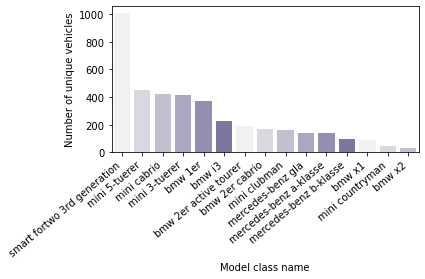
\includegraphics[width=.6\linewidth]{./Figures/fleet.png}
  \caption{Number of unique vehicles by class}
  \label{fig:Fleet}
\end{figure}

As can be seen in Figure \ref{fig:Fleet}, the number of vehicles of each type is far from equally distributed.
The dominant model in terms of number of vehicles is by a large margin the smart fortwo with 1007 unique vehicles, 
offering a high value proposition
in terms of parking space and ease of use for urban commuting. A clear tendency towards smaller cars, such as smarts
or minis is visible in the distribution.

\begin{figure}[htbp]
  \centering
  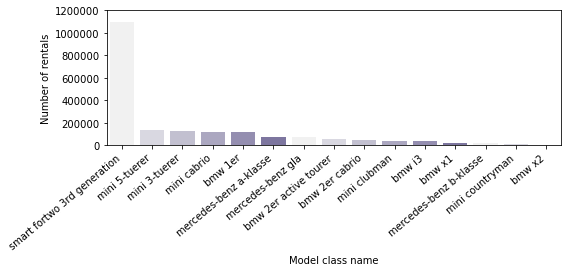
\includegraphics[width=.7\linewidth]{./Figures/travels.png}
  \caption{Number of rentals by class}
  \label{fig:Rentals}
\end{figure}

The actual amount of rentals, as shown in Figure \ref{fig:Rentals}, has a very similar order to the fleet size 
with only a few exceptions. Notably though, the smart has
seen even more demand than indicated by the number of vehicles.

The missing component however is the set of decidable classes. Similarly to the real world fleet deployment the
set of models is structured in terms of vehicle classes, namely $\mathbb{C} = \{ \text{XS}, \text{S}, \text{M}, \text{L} \}$.
Then each model was assigned to a class, the mapping can be found in Table \ref{table:VehicleClasses}.
These classes play an important role in the operational management of the car-sharing fleet since they differ in terms of costs and therefore profit.
 Additionally,  the cost function used in the simulation stage
of the framework is defined, based on the actual minute based pricing model of SHARE NOW. Although SHARE NOW also offers other tariffs, a focus was made on
the on-demand minute based charge system for this implementation \cite{ShareNowPricing}. The resulting function can be found in Table \ref{table:CostFunction}.

\subsection{Data preparation}
\label{sub_sec:CaseStudy/Preparation}

Before the actual classifier could be trained, the data had to be prepared to adhere to the form
required by the framework. Using the census data an area description for each request was
build where the set of categories to be analyzed includes the age distribution as well as the martial status.
$\mathbb{X} = \{ \text{Age}, \text{Marital Status} \}$. Then ranges for each were defined as can be seen in Table \ref{table:Ranges}.
Subsequently, rows with missing of malformed data were removed.

In early training iterations another important imbalance in the dataset was discovered. Classification models
trained on the data had a tendency to favor the "XS" class since there were far more rentals done with
vehicles from that class, since the set of features was missing an indicator for availability
of vehicles. To counteract that the data for each class was shuffled and truncated in such a way that
$\frac{nv(c_a)}{nv(c_b)} = \frac{nd(c_a)}{nd(c_b)} \ \forall c_a, c_b \in \mathbb{C}$, where $nv: \mathbb{C} \to \mathbb{N}$ is a function
that returns the number of vehicles of a specific category and $nd: \mathbb{C} \to \mathbb{N}$ is a function that returns the
amount of datapoints in the training set for each category. Reducing the impact of the availability of vehicles for
the classification task.

\subsection{Classifier}
\label{sub_sec:CaseStudy/Classifier}

Resulting in a dataset that mapped the framework definition of the customer request onto the class that the customer choose.
That data was then normalized into a zero to one range and split into a
training and a testing set and a Complement Naive Bayes classifier (CNB) was fit using
the training data. A Complement Naive Bayes Classifier is an adaption of a Multinomial Naive Bayes classifier, most
prominently known from text classification tasks \cite{rennie2003tackling}. Additionally, the CNB typically has an advantage when dealing
with imbalanced dataset such as ours.


\subsection{Simulation}
\label{sub_sec:CaseStudy/Simulation}

\begin{figure}[htbp]
  \centering
  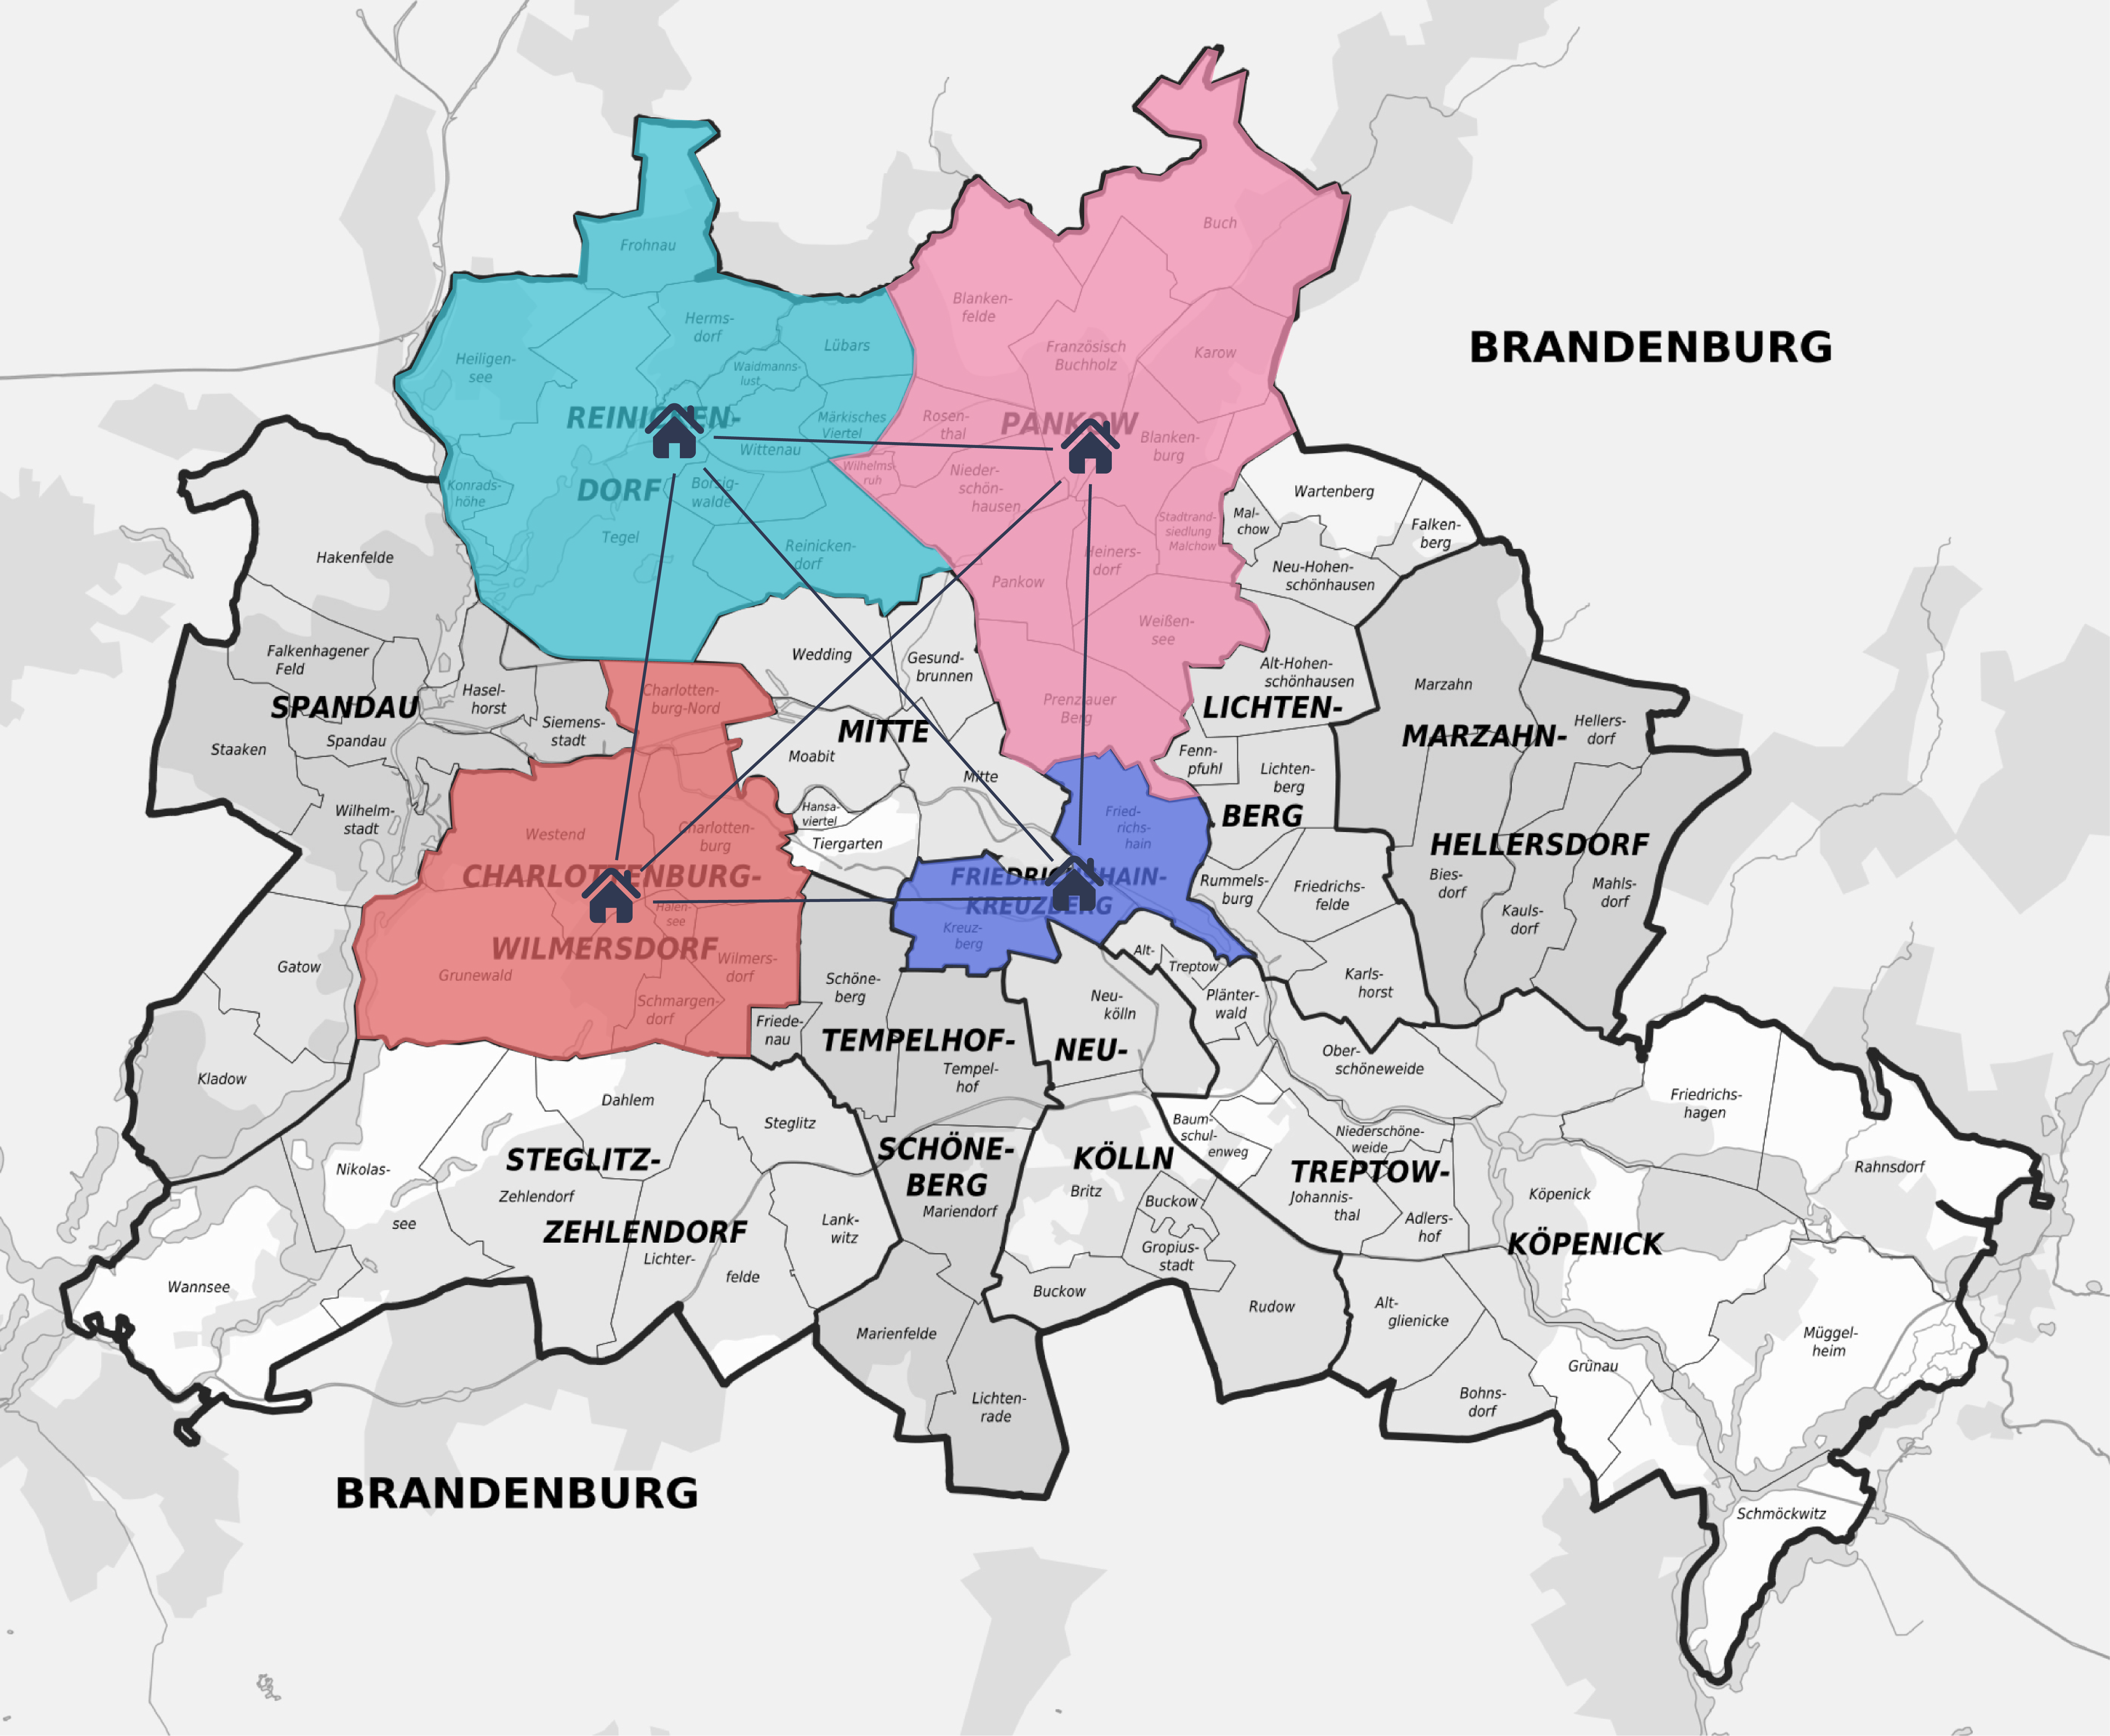
\includegraphics[width=.5\linewidth]{./Figures/graph.png}
  \caption{Simulation Graph}
  \label{fig:Graph}
\end{figure}
Before the actual implementation of the simulation stage, some data had to be prepared. Firstly 
the set of stations was to be defined, setting up the real world context of the simulation 
framework. Since the data was sourced in the city of Berlin, the simulation will also take place
in that setting. Firstly the area data regarding the age and marital status where sourced for various
districts in Berlin, as can be seen in Table \ref{table:Districts}. Then a subset of these were selected
to contain stations of our proposed simulation framework. This then forms our simulation graph as can be
seen in Figure \ref{fig:Graph}.


Afterwards the distance function $L: \mathbb{E} \to \mathbb{R}$ was determined for each edge in the proposed graph and can be found
in Table \ref{table:Distance}. Using this the set of stations $\mathbb{S} = \{ \text{Pankow}, \text{Reinickendorf}, \text{Kreuzberg}, \text{Charlottenburg} \}$ can be defined,
where the area function is the identity function. 

\begin{figure}[htbp]
  \centering
  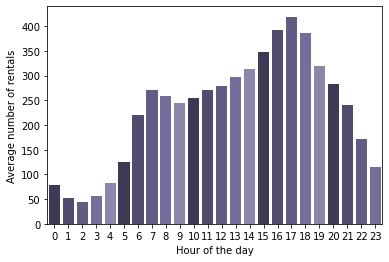
\includegraphics[width=.5\linewidth]{./Figures/hourly-demand.png}
  \caption{Average hourly demand of selected districts}
  \label{fig:Demand}
\end{figure}

Secondly, the simulation stage also requires the average time-period between customer arrivals for each working hour.
This was computed based on the dataset, by extracting datapoints which happened in the simulation areas $\mathbb{S}$ 
and grouping into days and then taking the average for each hour. The resulting
demand distribution can be seen in Figure \ref{fig:Demand}. The time period $p_h \ \forall h \in [0, 34] \subset \mathbb{N}$
can then be determined by $p_h = \frac{1}{\text{demand}_h}$ where $\text{demand}_h$ are the values from the figure.
Additionally, the value of $AS$ the average speed of urban commute was determined from the dataset to be $AS = 126.39 \frac{\text{m}}{\text{min}}$.

Using this information and the classifier described in Section \ref{sub_sec:CaseStudy/Classifier}, the simulation environment
was build in Python 3.10 using the SimPy library. The simulation receives the parameters $\alpha, C$ (Substitution Effect, Capacity),
the set of stations to be simulated, the hourly demand as well as the predictor function. That way different kind of classifiers
could be trained to quickly assess the performance of different classification models. 